\subsection{Secção biquadrática Tow-Tomas}
\subsubsection{Análise Teórica}

Na segunda parte da primeira sessão é estudada uma secção biquadrática TT, cujo esquema elétrico é apresentado na Fig. \ref{fig:tow_thomas_montagem}. Para a análise desta secção quadrática é ainda utilizado um circuito elementar adicional designado de integrador de Miller, cujo esquema está apresentado na Fig. \ref{fig:miller}, que corresponde a uma variação do integrador inversor apresentado na Fig. \ref{fig:circuitosElemnatres}. A resposta de um integrador de Miller é bem conhecida e dada por 
\begin{equation}\label{eq:miller}
    V_o(s)=-\frac{R_F||\frac{1}{Cs}}{R}V_I(s) = -\frac{R_F/R}{1+R_FCs}V_I(s)\:.
\end{equation}
\begin{figure}[h!]
    \centering
    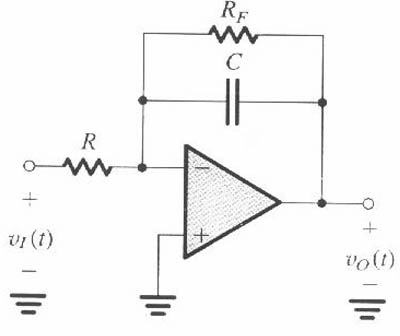
\includegraphics[width = 0.3\textwidth]{Imagens/miller.jpg}
    \caption{Integrador de Miller.}
    \label{fig:miller}
\end{figure}

\begin{figure}[h!]
    \centering
    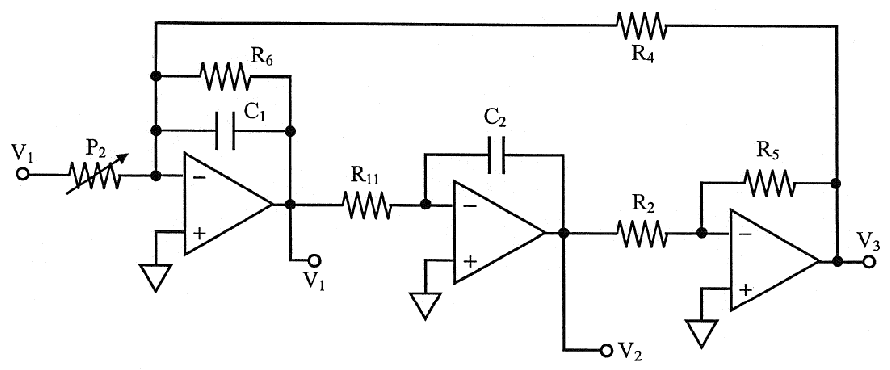
\includegraphics{Imagens/tow_thomas_montagem.pdf}
    \caption{Secção biquadrática de Tow-Thomas (TT).}
    \label{fig:tow_thomas_montagem}
\end{figure}

Utilizando o circuito elementar do integrador inversor \eqref{eq:int_inv}, analisando a secção biquadrática TT, obtém-se
\begin{equation}\label{eq:TTeq1}
    V_2(s) = -\frac{1}{R_{11}C_2s}V_1(s)  \Rightarrow \frac{V_2(s)}{V_1(s)} = -\frac{1}{R_{11}C_2s}\:.
\end{equation}
Para além disso, fazendo uso do circuito elementar multiplicador-inversor \eqref{eq:multInv} vem que 
\begin{equation}\label{eq:TTeq2}
    V_3(s) = -\frac{R_5}{R_2}V_2(s) \Rightarrow \frac{V_3(s)}{V_2(s)} = -\frac{R_5}{R_2}\:.
\end{equation}
Por fim, utilizando o teorema da sobreposição e o circuito elementar do integrador de Miller \eqref{eq:miller} obtém-se
\begin{equation}\label{eq:TTeq3}
    V_1(s) = -\frac{R_6/P_2}{1+R_6C_1s}V_i(s) -\frac{R_6/R_4}{1+R_6C_1s}V_3(s)\:.
\end{equation}
Manipulando as equações \eqref{eq:TTeq1}, \eqref{eq:TTeq2}, e \eqref{eq:TTeq3} obtêm-se as funções de transferência 
\begin{equation}\label{eq:TTeq1M}
    T_1(s) = \frac{V_1(s)}{V_i(s)} = -\frac{\frac{1}{P_2C_1}s}{s^2+\frac{1}{R_6C_1}s+\frac{R_5}{R_2}\frac{1}{R_{4}R_{11}C_1C_2}}\:,
\end{equation}
\begin{equation}\label{eq:TTeq2M}
    T_2(s) = \frac{V_2(s)}{V_i(s)} = \frac{\frac{1}{P_2R_{11}C_1C_2}}{s^2+\frac{1}{R_6C_1}s+\frac{R_5}{R_2}\frac{1}{R_{4}R_{11}C_1C_2}} \:,
\end{equation}
e
\begin{equation}\label{eq:TTeq3M}
  T_3(s) = \frac{V_3(s)}{V_i(s)} = -\frac{\frac{R_5}{R_2}\frac{1}{P_2R_{11}C_1C_2}}{s^2+\frac{1}{R_6C_1}s+\frac{R_5}{R_2}\frac{1}{R_{4}R_{11}C_1C_2}}\:.
\end{equation}
Em primeiro lugar, $T_1(s)$ tem um zero na origem, ganho estático nulo, \textit{i.e.}, $\lim_{\omega \rightarrow 0} T_1(j\omega) = 0$, e atenua as altas frequências, \textit{i.e.}, $\lim_{\omega \rightarrow \infty} T_1(j\omega) = 0$. Por estas razões, $T_1(s)$ é passa-banda. Em segundo lugar, $T_2(s)$ e $T_3(s)$ não têm zeros, têm ganho estático não nulo, \textit{i.e.}, $\lim_{\omega \rightarrow 0} T_2(j\omega) = K$ e $\lim_{\omega \rightarrow 0} T_2(j\omega) = GK$, e atenua as altas frequências, \textit{i.e.}, $\lim_{\omega \rightarrow \infty} T_2(j\omega) = 0$. Por estas razões, $T_2(s)$ e $T_3(s)$ são ambos passa-baixo. 

Tendo em consideração o denominador das funções transferência é possível construir um modelo que possa ser descrito por um DFS semelhante ao da Fig. \ref{fig:dfs_KHN} para a secção KHN. De facto, tal é possível tentando modelar cada uma das três funções transferência como 
\begin{equation}\label{eq:TTeq1MM}
    T_1(s) = \frac{K\omega_0s}{s^2+(\omega_0/Q)s-G\omega_0^2}\:, 
\end{equation}
\begin{equation}\label{eq:TTeq2MM}
    T_2(s) = \frac{K\omega_0^2}{s^2+(\omega_0/Q)s-G\omega_0^2} \:,
\end{equation}
e
\begin{equation}\label{eq:TTeq3MM}
    T_3(s) = \frac{KG\omega_0^2}{s^2+(\omega_0/Q)s-G\omega_0^2}\:.
\end{equation}
Comparando as equações \eqref{eq:TTeq1M},\eqref{eq:TTeq2M}, e \eqref{eq:TTeq3M} com as equações \eqref{eq:TTeq1MM},\eqref{eq:TTeq2MM}, e \eqref{eq:TTeq3MM}, obtemos 
\begin{align}
    \frac{1}{P_2C_1} = K\omega_0\;, \quad \frac{1}{R_6C_1} = \frac{\omega_0}{Q}\;, \quad \frac{R_5}{R_2}\frac{1}{R_{4}R_{11}C_1C_2} = - G\omega_0^2\;,\\ \frac{1}{P_2R_{11}C_1C_2} = K \omega_0^2\;, -\frac{R_5}{R_2}\frac{1}{P_{2}R_{11}C_1C_2} = GK\omega_0^2\:,
\end{align}
que resolvendo em ordem a $\omega_0$, $K$, $Q$, e $G$ resulta, respetivamente, em 
\begin{equation}\label{eq:w0TT}
    \omega_0 = \frac{1}{R_{11}C_2} = \frac{1}{\sqrt{R_4R_{11}C_1C_2}}\:,
\end{equation}
\begin{equation}\label{eq:KTT}
    K=\frac{R_{11}C_2}{P_2C_1}=\frac{R_4}{P_{2}}\:,
\end{equation}
\begin{equation}\label{eq:QTT}
    Q=\frac{R_6C_1}{R_{11}C_2}\:,
\end{equation}
e
\begin{equation}\label{eq:GTT}
    G=-\frac{R_5}{R_2}\:.
\end{equation}
Desta forma, o DFS equivalente é apresentado na Fig. \ref{fig:dfs_tow_thomas_montagem}.
\begin{figure}[h!]
    \centering
    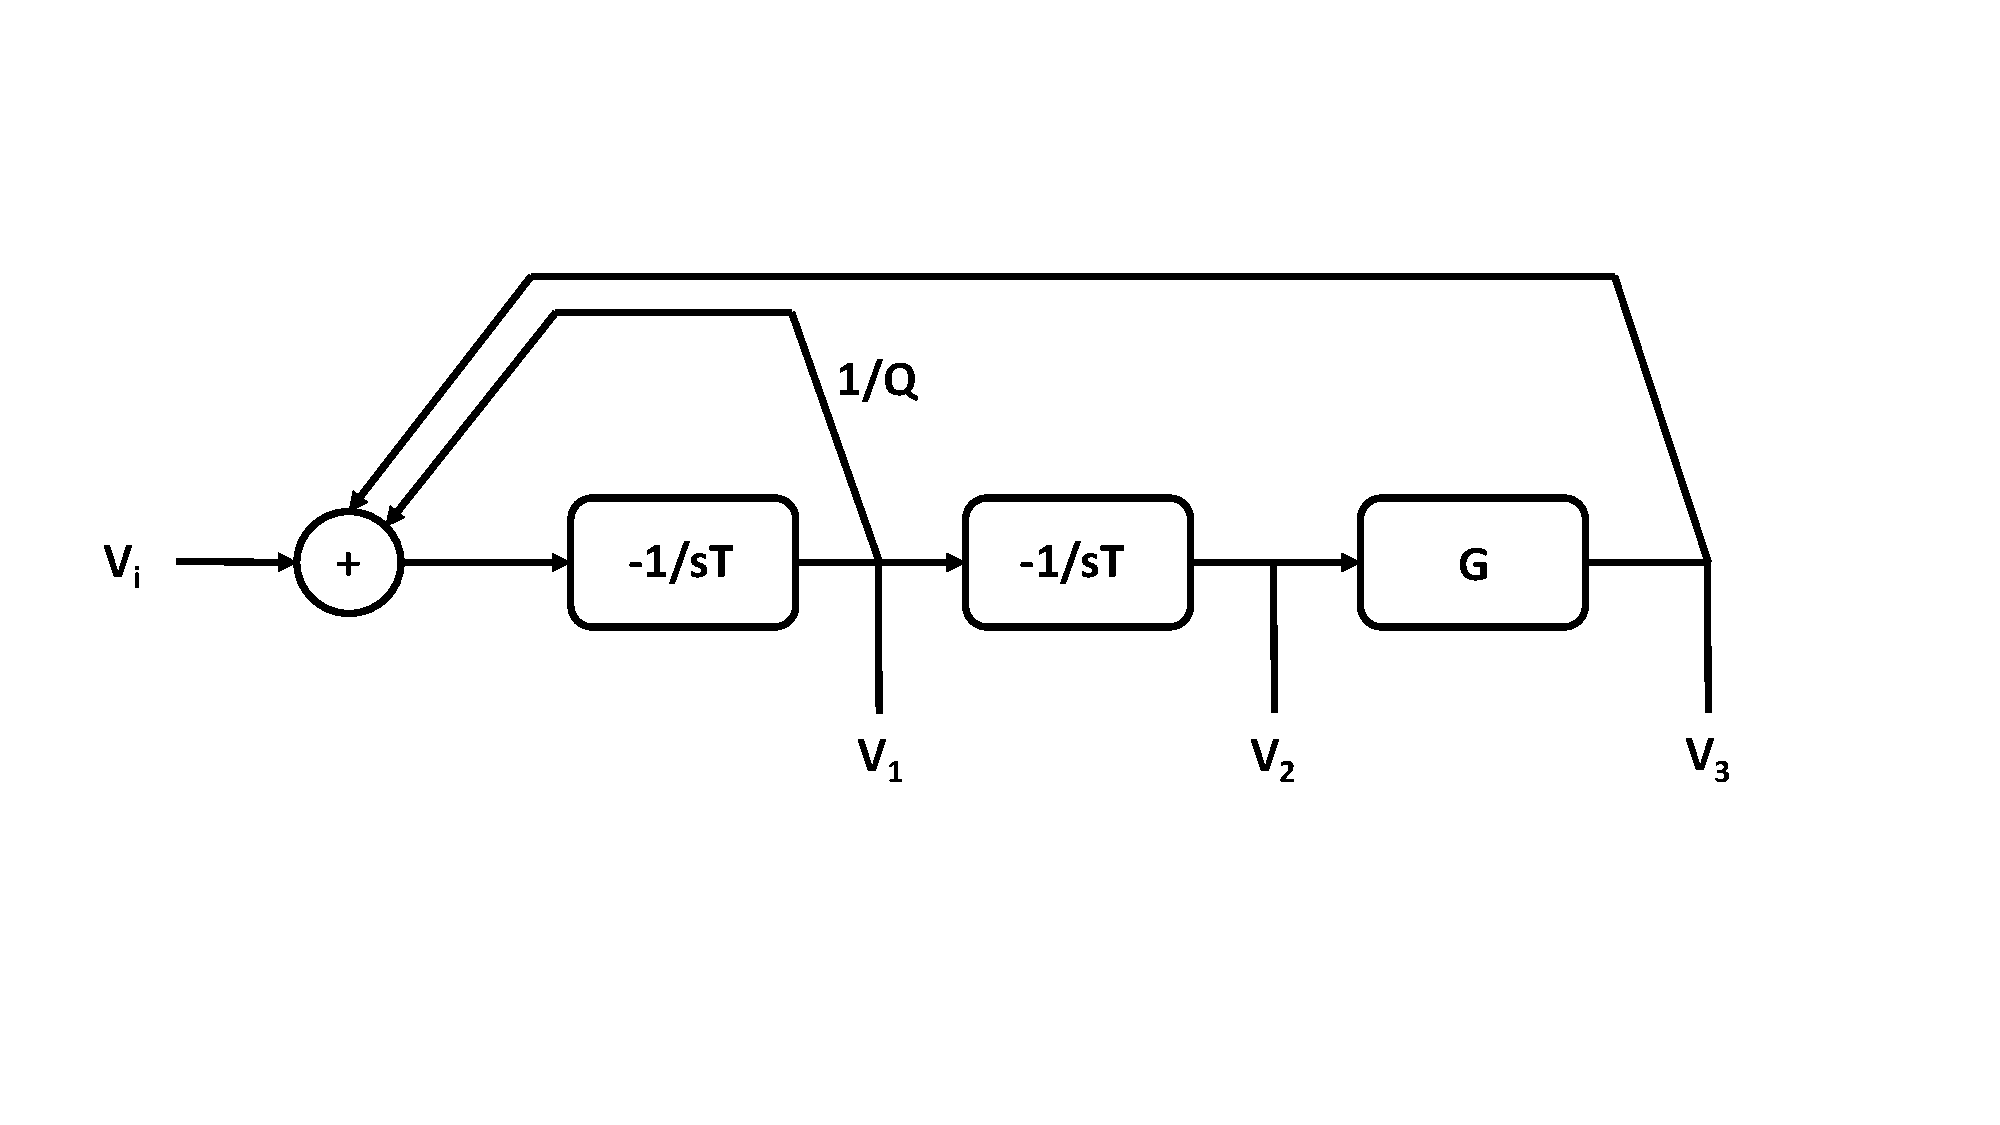
\includegraphics[width = 0.8\textwidth]{Imagens/dfs_TT.pdf}
    \caption{DFS da secção biquadrática de Tow-Thomas (TT).}
    \label{fig:dfs_tow_thomas_montagem}
\end{figure}

Substituindo os valores dos componentes indicados em \eqref{eq:w0TT}, \eqref{eq:KTT}, \eqref{eq:QTT}, e \eqref{eq:GTT} obtemos os valores teóricos de $\omega_0$, $K$, $Q$, e $G$ dos filtros TT utilizados na atividade laboratorial, apresentados na Tabela \ref{tab:parTT}. Verifica-se, ainda, que as condições entre valores dos componentes do circuito nas equações \eqref{eq:w0TT} e \eqref{eq:KTT} são verificadas.

\begin{table}[h!]
    \centering
        \caption{Valores teóricos de $\omega_0$, $K$,$Q$, e $G$ dos filtros TT, arredondados a 4 algarismos significativos.}
    \begin{tabular}{ccccc}
        \hline
         $\omega_0$ & $f_0$ & $Q$ & $K$ & $G$ \\
         \hline
         $2.128 \times 10^{4}$ rad/$\mathrm{s^{-1}}$ & 3.386 kHz & 1.000 & 1.000 & 1.000\\
          \hline
    \end{tabular}

    \label{tab:parTT}
\end{table}

Após o estudo do circuito para o valor total de $P_2$, estudou-se a sua resposta para diferentes valores, utilizando-o como uma resistência variável. De \eqref{eq:KTT} e \eqref{eq:QTT}, espera-se que $Q$ não varie com a variação de $P_2$ e que K seja inversamente proporcional a $P_2$ com constante $R_4$, tal como apresentado na Fig. \ref{fig:K_vs_P2_TT}. Dadas \eqref{eq:TTeq1MM}, \eqref{eq:TTeq2MM}, e \eqref{eq:TTeq3MM}, espera-se que as variações de K se traduzam em translações verticais dos diagramas de Bode obtidos, i.e., para menores valores de $P_2$, K aumenta e portanto os diagramas de Bode sofrem translações positivas verticais tal como ilustrado nas Fig. \ref{fig:TT1_Bode_variacao_P2}, \ref{fig:TT2_Bode_variacao_P2}, e \ref{fig:TT3_Bode_variacao_P2}. Também se pode observar como Q não se altera, pois Q altera o ganho dos filtros em torno da frequência $\omega_0$ e a variação que se pode detetar é apenas a translação vertical já mencionada e que se deve a K. Assim, os efeitos da variação de $P_2$ são facilmente ilustrados pelo ganho a baixas frequências dos filtros passa-baixo para K e pelo ganho à frequência central do filtro passa-banda para Q.

\begin{figure}[ht]
     \begin{subfigure}[b]{0.45\textwidth}
        \centering
        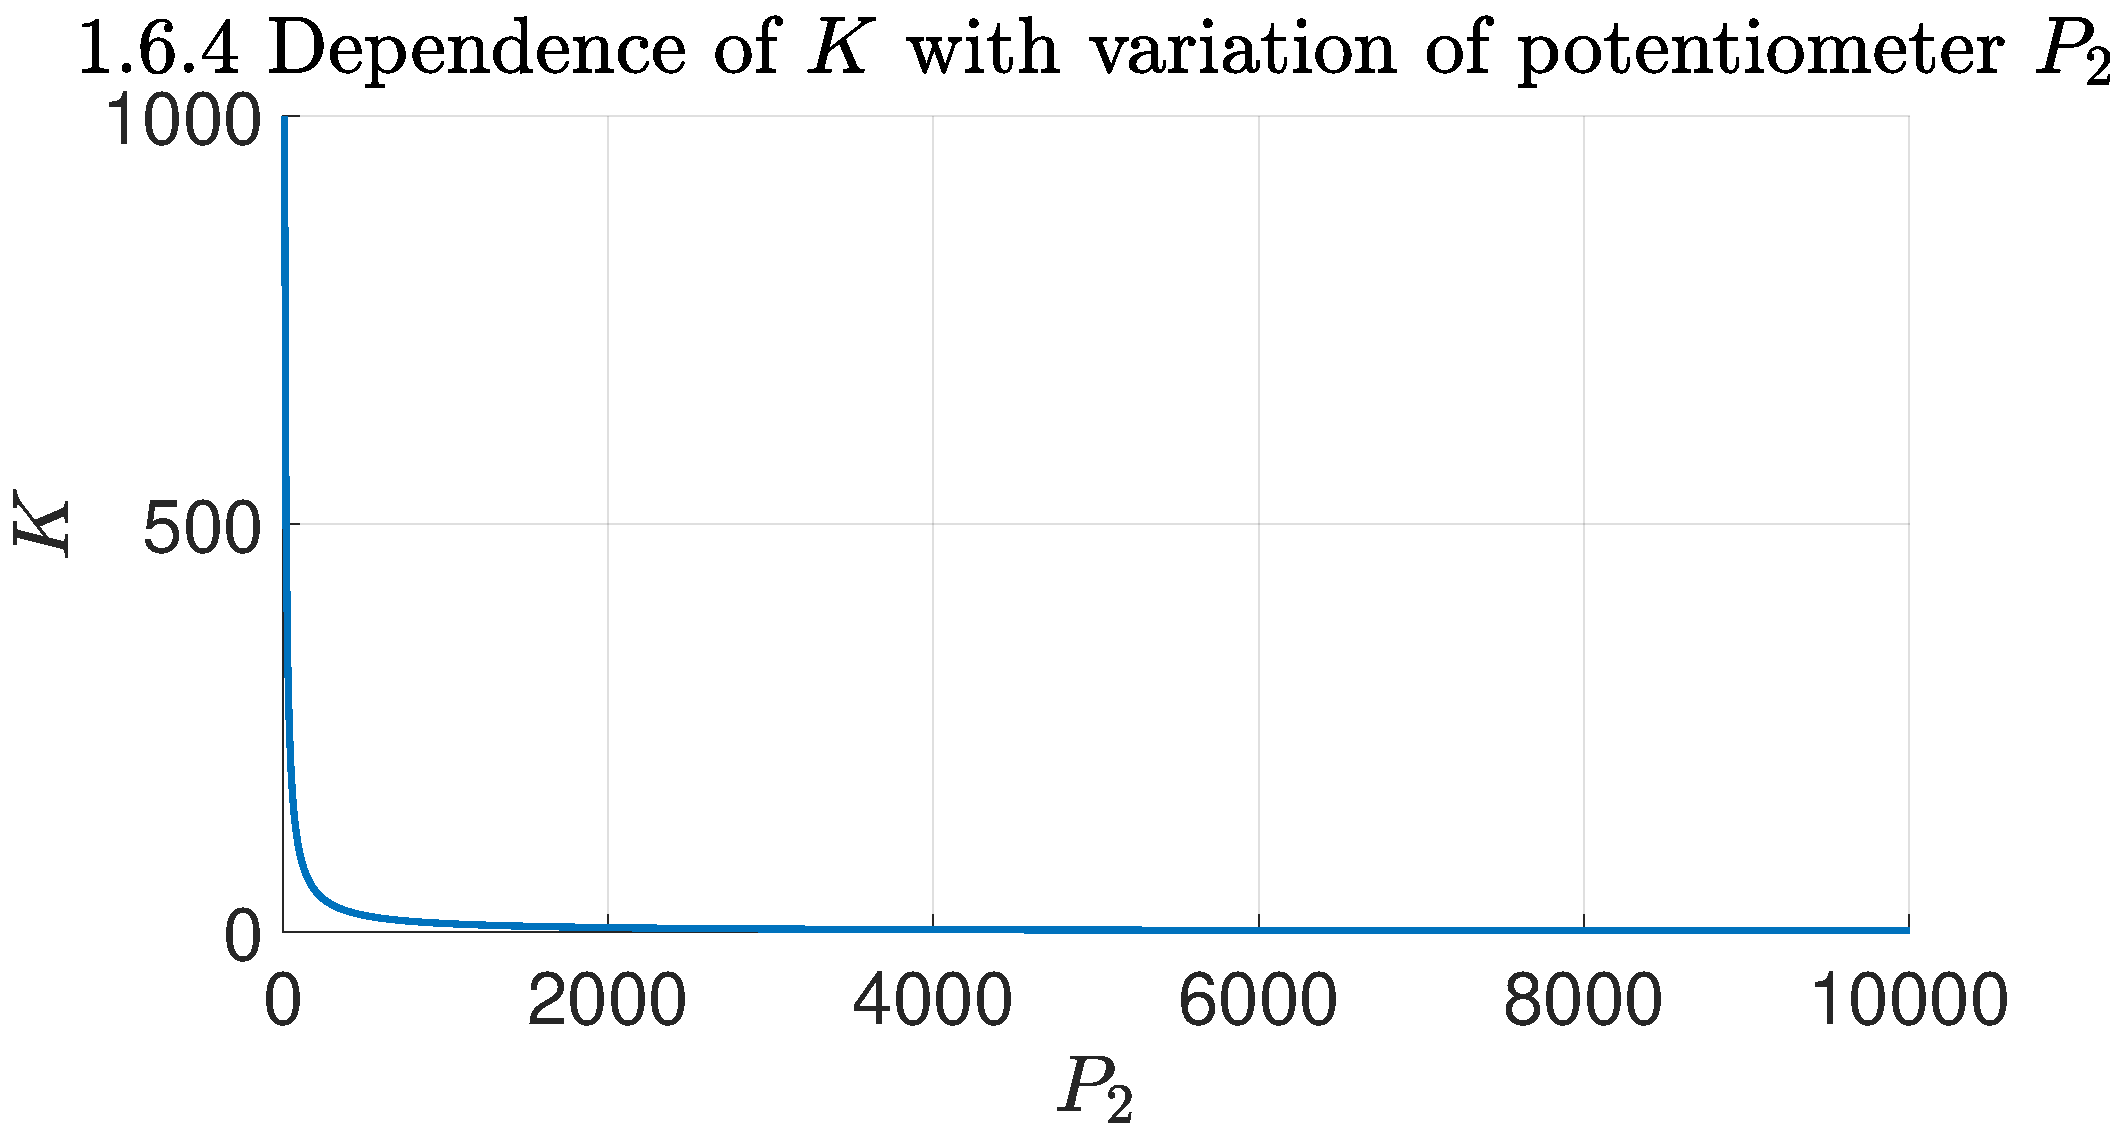
\includegraphics[width=\linewidth]{Imagens/1_6_4_GainPotentiometer3.pdf}
        \caption{Relação de K e $P_2$ na montagem de TT.}
        \label{fig:K_vs_P2_TT}
     \end{subfigure}
     \hfill
     \begin{subfigure}[b]{0.45\textwidth}
         \centering
         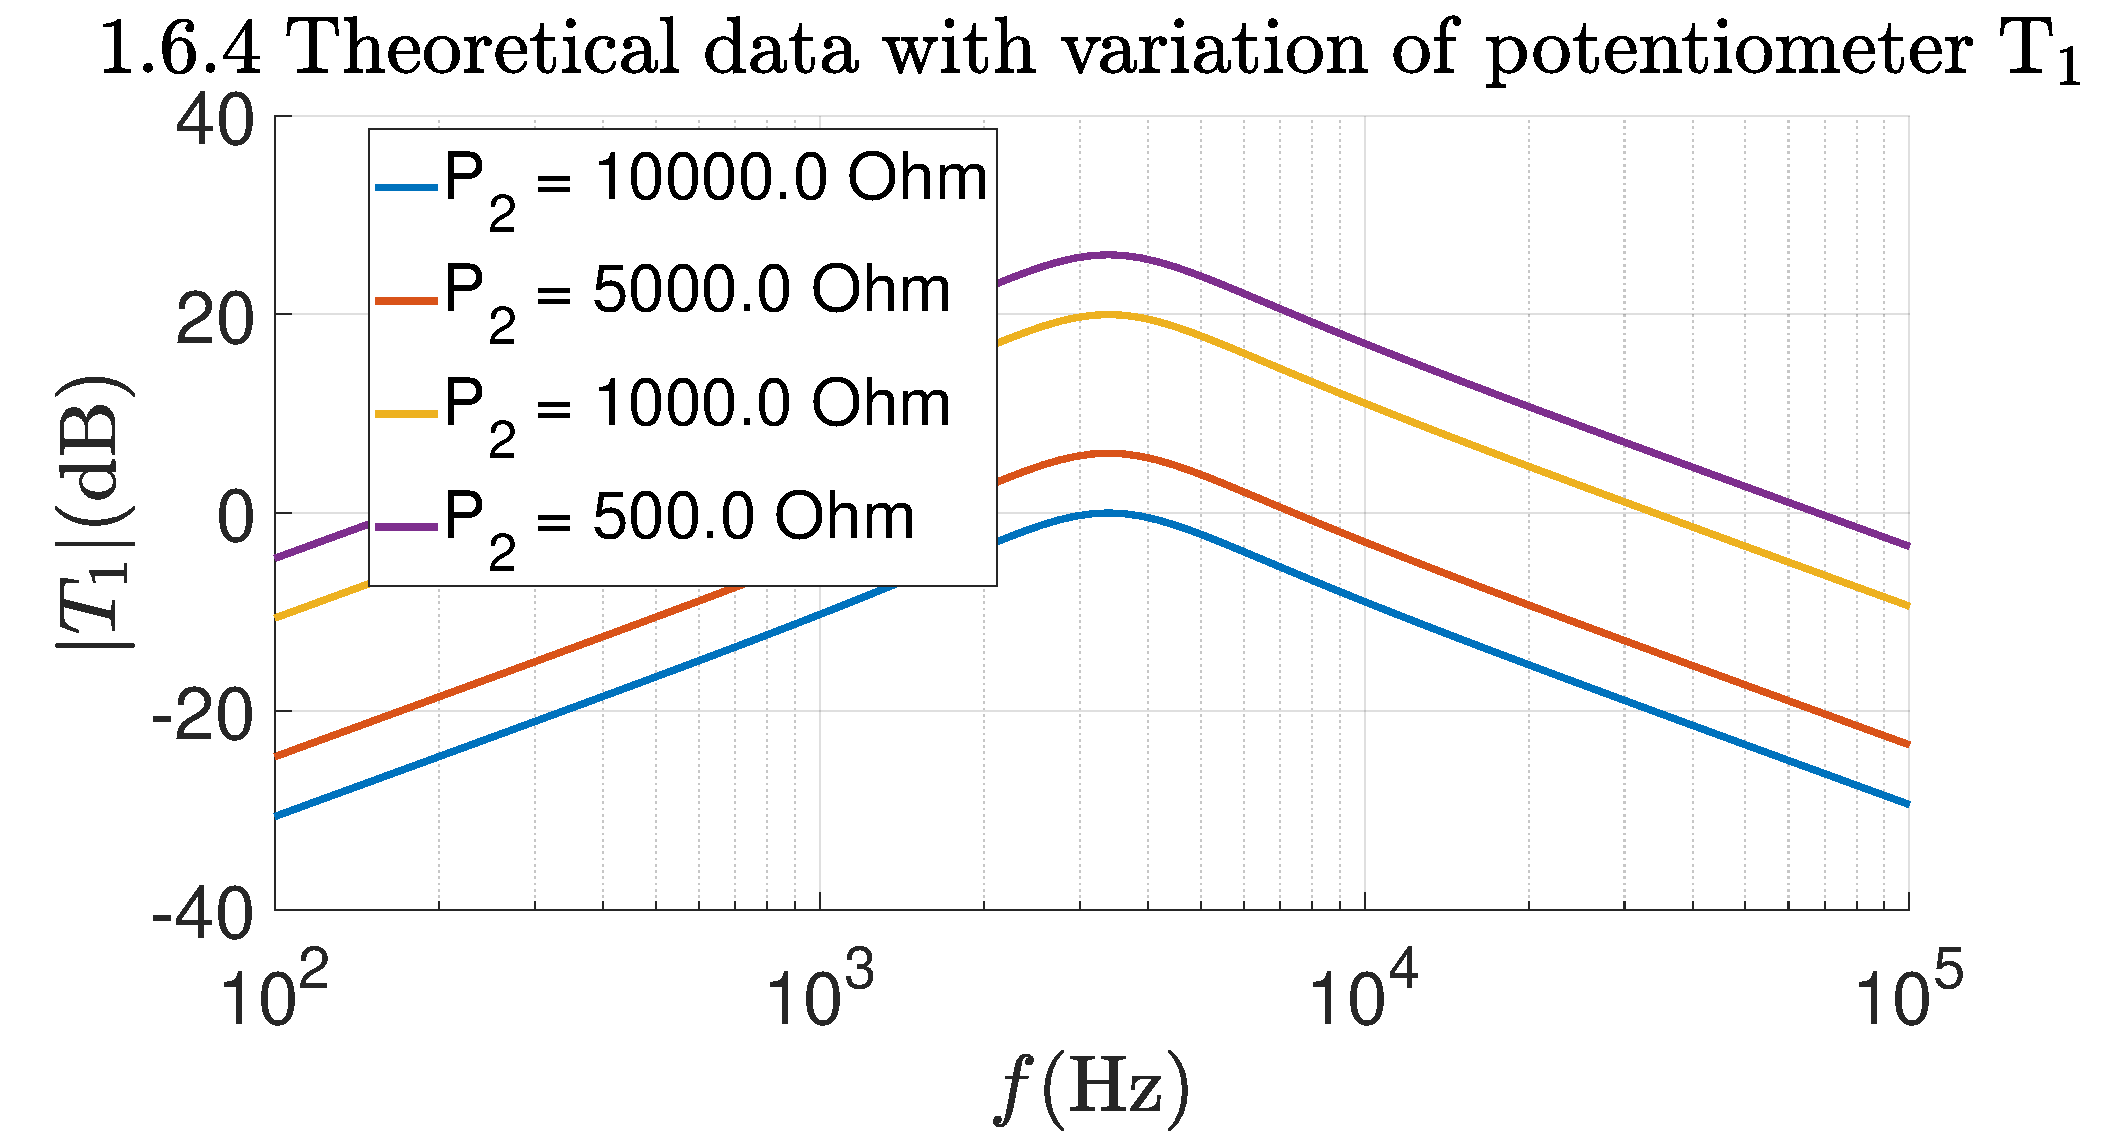
\includegraphics[width=\textwidth]{Imagens/1_6_4_bodeTheoreticalPotentiometer1.pdf}
         \caption{Filtro $T_1$ para vários valores de $P_2$.}
         \label{fig:TT1_Bode_variacao_P2}
     \end{subfigure}

     \begin{subfigure}[b]{0.45\textwidth}
         \centering
         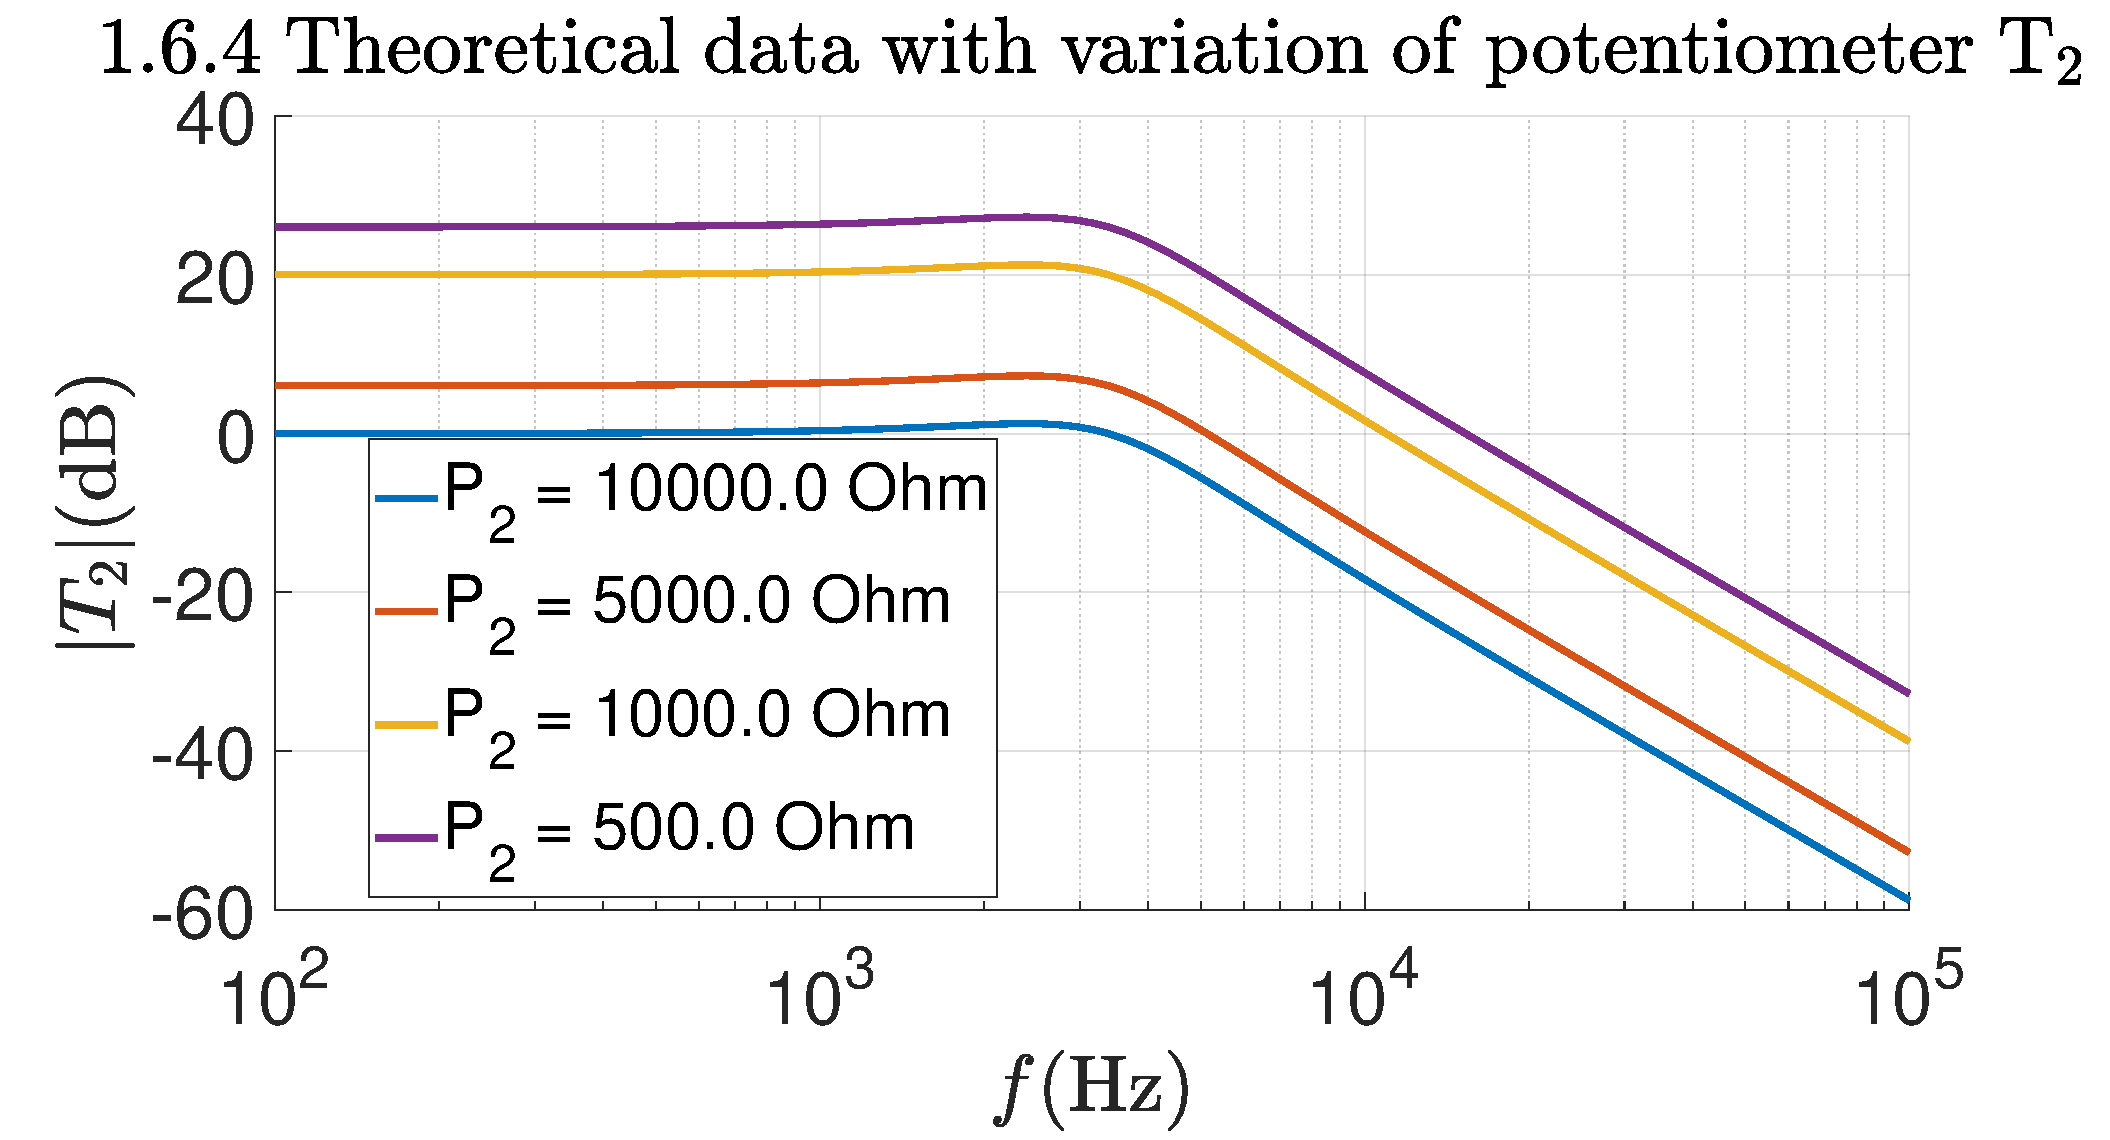
\includegraphics[width=\textwidth]{Imagens/1_6_4_bodeTheoreticalPotentiometer2.pdf}
         \caption{Filtro $T_2$ para vários valores de $P_2$.}
         \label{fig:TT2_Bode_variacao_P2}
     \end{subfigure}
     \hfill
     \begin{subfigure}[b]{0.45\textwidth}
         \centering
         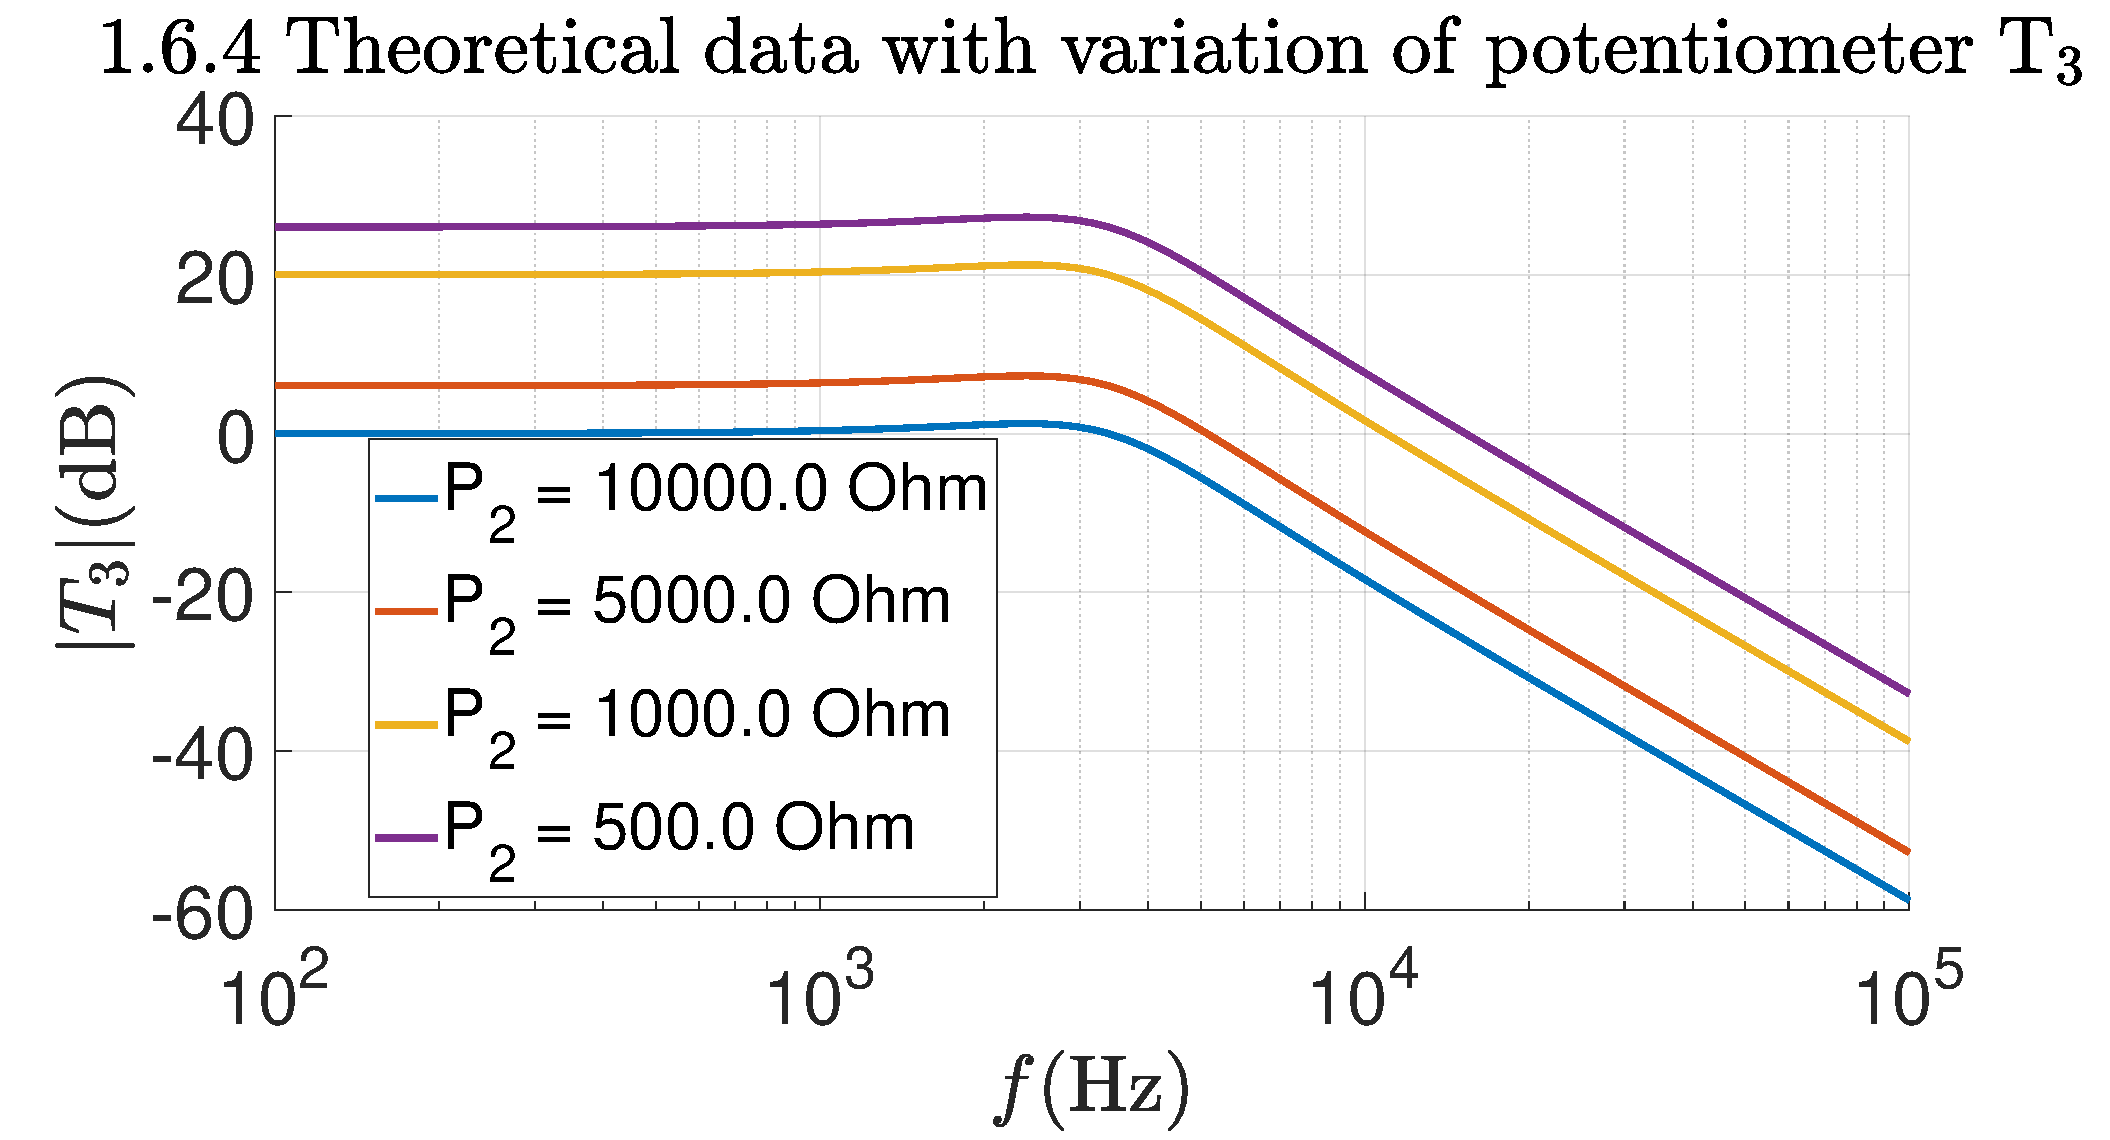
\includegraphics[width=\textwidth]{Imagens/1_6_4_bodeTheoreticalPotentiometer3.pdf}
         \caption{Filtro $T_3$ para vários valores de $P_2$.}
         \label{fig:TT3_Bode_variacao_P2}
     \end{subfigure}
    \caption{Efeitos da variação de $P_2$ sobre $K$ e as respostas dos filtros.}
\end{figure}

\subsubsection{Trabalho Experimental}
Realizou-se no módulo experimental a montagem esquematizada na Fig. \ref{fig:tow_thomas_montagem}, utilizando o valor total de $P_2$. A frequência central do filtro passa-banda ocorre para uma diferença de fase de $180 \degree$, tendo-se assim determinado $f_0 = 3.80 \si{\kilo \hertz}$. As frequências de corte deste filtro obtiveram-se para diferenças de fase de $225 \degree$ e $135 \degree$, chegando-se a $f_{c1} = 2.34 \si{\kilo \hertz}$ e $f_{c2} = 6.20 \si{\kilo \hertz}$. Estes valores de frequência entre outros foram utilizados para a obtenção dos diagramas de Bode experimentais, estando registados na Tabela \ref{tab:dados_bode_exp_TT} juntamente com os correspondentes valores de tensão ($V_1$, $V_2$, e $V_3$) e os valores de ganho de cada filtro ($\left |T_1(j\omega)\right|$, $\left |T_2(j\omega)\right|$, e $\left |T_3(j\omega)\right|$). É de notar que todas estas medições foram realizadas para $V_i = 2.15 \si{\volt}$ e obtidas com o osciloscópio, que permite uma maior exatidão na sua determinação.

\begin{table}[ht]
    \centering
    \caption{Valores experimentais das tensões de saída e dos ganhos da secção biquadrática de Tow-Thomas.}
    \begin{tabular}{ccccccc}
        \hline
        $f [\si{\kilo \hertz}]$ & $V_1 [\si{\volt}]$ & $\left |T_1 (j \omega) \right| [\si{\decibel}]$ & $V_2 [\si{\volt}]$ & $\left |T_2 (j \omega) \right| [\si{\decibel}]$ & $V_3 [\si{\volt}]$ & $\left |T_3 (j \omega) \right| [\si{\decibel}]$\\
        \hline
        0.500   & 0.271 & -18.0 & 2.15  & 0.00  & 2.15  & 0.00 \vspace{0.2cm}\\
        1.38    & 0.830 & -8.27 & 2.25  & 0.395  & 2.29  & 0.548  \vspace{0.2cm}\\
        2.34    & 1.51  & -3.07 & 2.40  & 0.956  & 2.40  & 0.956  \vspace{0.2cm}\\
        3.80    & 2.13  & -0.0812& 2.17  & 0.0804 & 2.17  & 0.0804 \vspace{0.2cm}\\
        6.20    & 1.51 & -3.07 & 0.997 & -6.67 & 1.036 & -6.31 \vspace{0.2cm}\\
        8.72    & 1.04  & -6.31 & 0.490 & -12.8 & 0.510 & -12.5 \vspace{0.2cm}\\
        20.0    & 0.400 & -14.6 & 0.090 & -27.6 & 0.118 & -25.2 \vspace{0.2cm}\\
        \hline
    \end{tabular}
    \label{tab:dados_bode_exp_TT}
\end{table}

Dos valores da Tabela \ref{tab:dados_bode_exp_TT} pode-se, assim, calcular os valores de $K$, $\omega_0$, $Q$, e $G$. $K$ pode ser obtido, de acordo com \eqref{eq:TTeq3MM} como o ganho a baixas frequências do filtro $T_3$, ou seja, $K \approx 2.15/2.15 = 1.00$. $G$ pode ser obtido, de acordo com \eqref{eq:TTeq2MM}, dividindo $K$ pelo ganho a baixas frequências do filtro $T_2$, ou seja, $G \approx 1.00/(2.15/2.15) = 1.00$. Por sua vez, $\omega_0$ obtém-se como $\omega_0 = 2 \pi f_0 \approx 23.9 \times 10^3 \si{\radian\per\second}$. Finalmente, de \eqref{eq:TTeq1MM} pode-se escrever
\begin{equation*}
    \left |T_1 (j \omega_0) \right| = \frac{K}{\sqrt{(G-1)^2 + \frac{1}{Q}}} \Leftrightarrow Q = \sqrt{\frac{1}{\frac{K^2}{\left |T_1 (j \omega_0) \right|^2} - (G-1)^2}} \approx 0.991.
\end{equation*}
Estes valores estão resumidos na Tabela \ref{tab:valores_teoricos_experimentais_TT}.

Os valores de $K$, $Q$, e $\omega_0$ podem também ser obtidos através de um método de mínimos quadrados de adaptação da curva de $\left |T_1 (j\omega)\right|$ descrita por \eqref{eq:TTeq1MM} aos dados experimentais tal como ilustrado na Fig. \ref{fig:adaptacao}. Com este método, onde se considera $G \approx 1.00$ como determinado experimentalmente acima, obteve-se os valores da Tabela \ref{tab:estimativas_LSQ_TT}. Estes valores estão próximos dos determinados pelo método anterior e a utilização de ambos reforça a sua validade. No entanto, para comparação com os valores teóricos serão utilizados os valores obtidos com o método anterior.

\begin{figure}[ht]
    \centering
    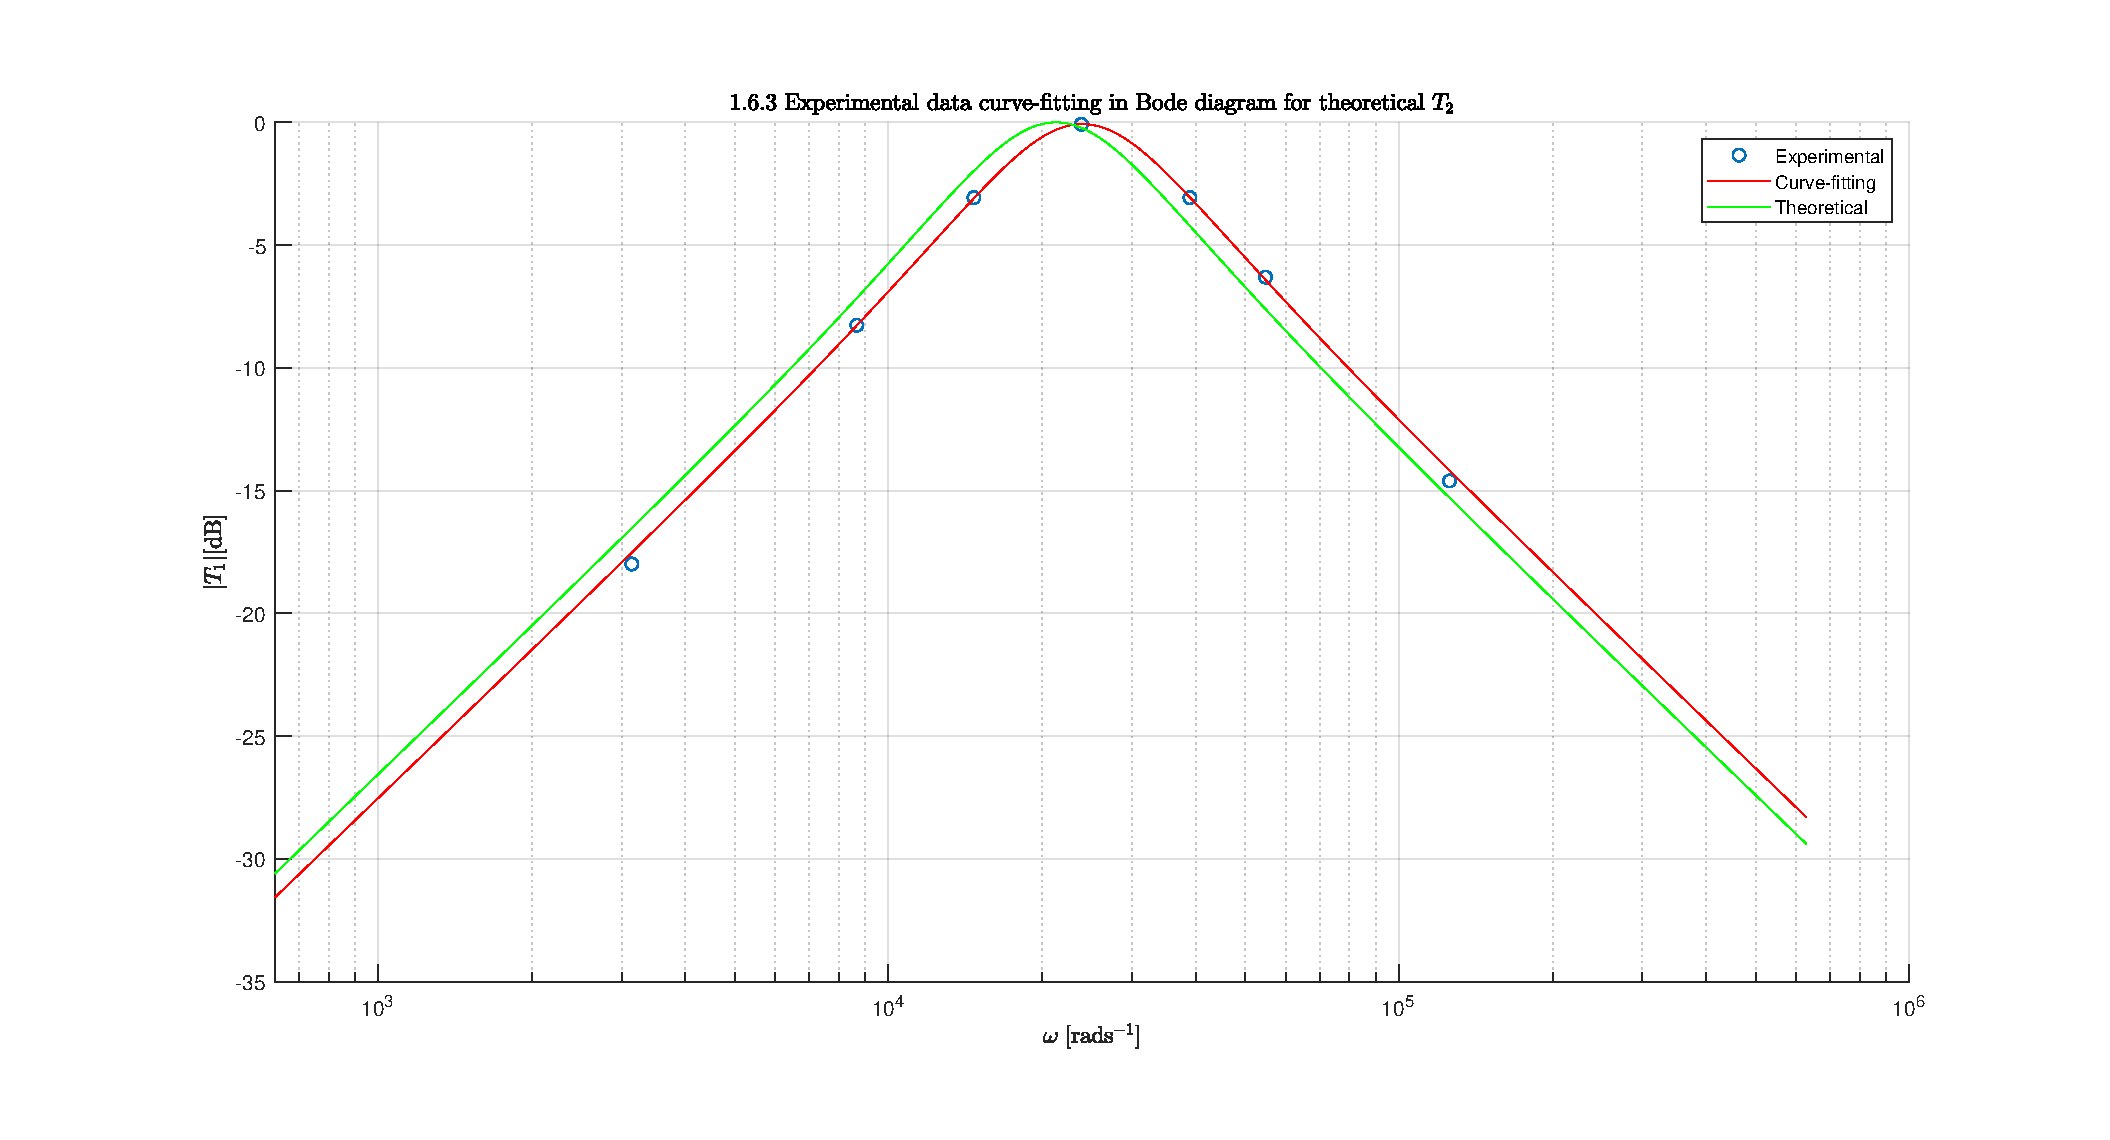
\includegraphics[width=\linewidth]{Imagens/adaptacao_bode_experimental_T1.pdf}
    \caption{Adaptação de uma curva de acordo com $T_2$ teórica aos resultados experimentais.}
    \label{fig:adaptacao}
\end{figure}

\begin{table}[ht]
    \centering
    \caption{Valores experimentais obtidos com o método dos mínimos quadrados para os parâmetros da TT.}
    \begin{tabular}{ccccccc}
    \hline
    Parâmetro & Valor estimado com os mínimos quadrados \\
    \hline  
    $K$ & 1.01 \\
    $Q$ & 0.985 \\
    $\omega_0 [\si{\radian\per\second}]$ & $24.0\times10^3$ \\
    \hline
    \end{tabular}
    \label{tab:estimativas_LSQ_TT}
\end{table}

Após as experiências com o valor constante e total de $P_2$, estudou-se também a influência da sua variação sobre os parâmetros da resposta, $K$, $Q$, e $\omega_0$. Com esse intuito, retiraram-se os dados registados nas Tabelas \ref{tab:influencia_P2_TT_V1} e \ref{tab:influencia_P2_TT_V2}. Os valores de \ref{tab:influencia_P2_TT_V2} ilustram o ganho do filtro $T_2$ a baixas frequências sendo portanto dependentes do K e não de Q, pois o filtro $T_2$ é passa-baixo. Os valores de \ref{tab:influencia_P2_TT_V1} são utilizados para mostrar como varia o ganho na zona de passagem do filtro passa-banda, pois esses valores são dependentes de $Q$ e de $K$. Em conjunto estas tabelas permitem inferir as consequências da variação do valor de $P_2$. É ainda de referir que se mediu o valor de $R_4$ com o multímetro no modo ohmímetro, tendo-se obtido $R_4 = 9.76 \si{\kilo \ohm}$.

\begin{table}[ht]
    \centering
    \caption{Valores experimentais da variação do valor de $P_2$.}
    \begin{subtable}[h]{0.45\textwidth}
        \centering
        \caption{Medições de $V_2$ e $\left |T_2 (j \omega) \right|$ para $f = 100 \si{\hertz}$.}
        \label{tab:influencia_P2_TT_V2}
        \begin{tabular}{ccccc}
            \hline
            $P_2 [\si{\kilo \ohm}]$ & $V_i [\si{\volt}]$ & $V_2 [\si{\volt}]$ & $\left |T_2 (j \omega) \right|$ & $R_4/P_2$ \\
            \hline
            4.95    & 1.09  & 2.13  & 1.95 & 1.97 \vspace{0.2cm}\\
            1.002   & 1.05  & 10.3  & 9.81 & 9.74  \vspace{0.2cm}\\
            0.496   & 1.01  & 18.7  & 18.5 & 19.7  \vspace{0.2cm}\\
            \hline
        \end{tabular}
    \end{subtable}
    \hfill
    \begin{subtable}[h]{0.45\textwidth}
        \centering
        \caption{Medições de $V_1$ e $\left |T_1 (j \omega) \right|$ para $f = 3.80 \si{\kilo \hertz}$.}
        \label{tab:influencia_P2_TT_V1}
        \begin{tabular}{cccc}
            \hline
            $P_2 [\si{\kilo \ohm}]$ & $V_i [\si{\volt}]$ & $V_2 [\si{\volt}]$ & $\left |T_1 (j \omega) \right|$ \\
            \hline
            4.95    & 1.09  & 2.13  & 1.95   \vspace{0.2cm}\\
            1.002   & 1.05  & 10.2  & 9.71   \vspace{0.2cm}\\
            0.496   & 1.01  & 18.9  & 18.7   \vspace{0.2cm}\\
            \hline
        \end{tabular}
    \end{subtable}
\end{table}

\subsubsection{Comparação de resultados}

Obteve-se os diagramas de Bode de amplitude ponto-a-ponto das Fig. \ref{fig:bode_exp_TT_P2_10kohm_T1}, \ref{fig:bode_exp_TT_P2_10kohm_T2} e \ref{fig:bode_exp_TT_P2_10kohm_T3}. De acordo com elas, observa-se em primeiro lugar que os resultados experimentais da montagem TT se ajustam bem em termos de diagramas de Bode aos resultados teóricos. 
\begin{figure}[ht]
     \begin{subfigure}[b]{0.45\textwidth}
         \centering
         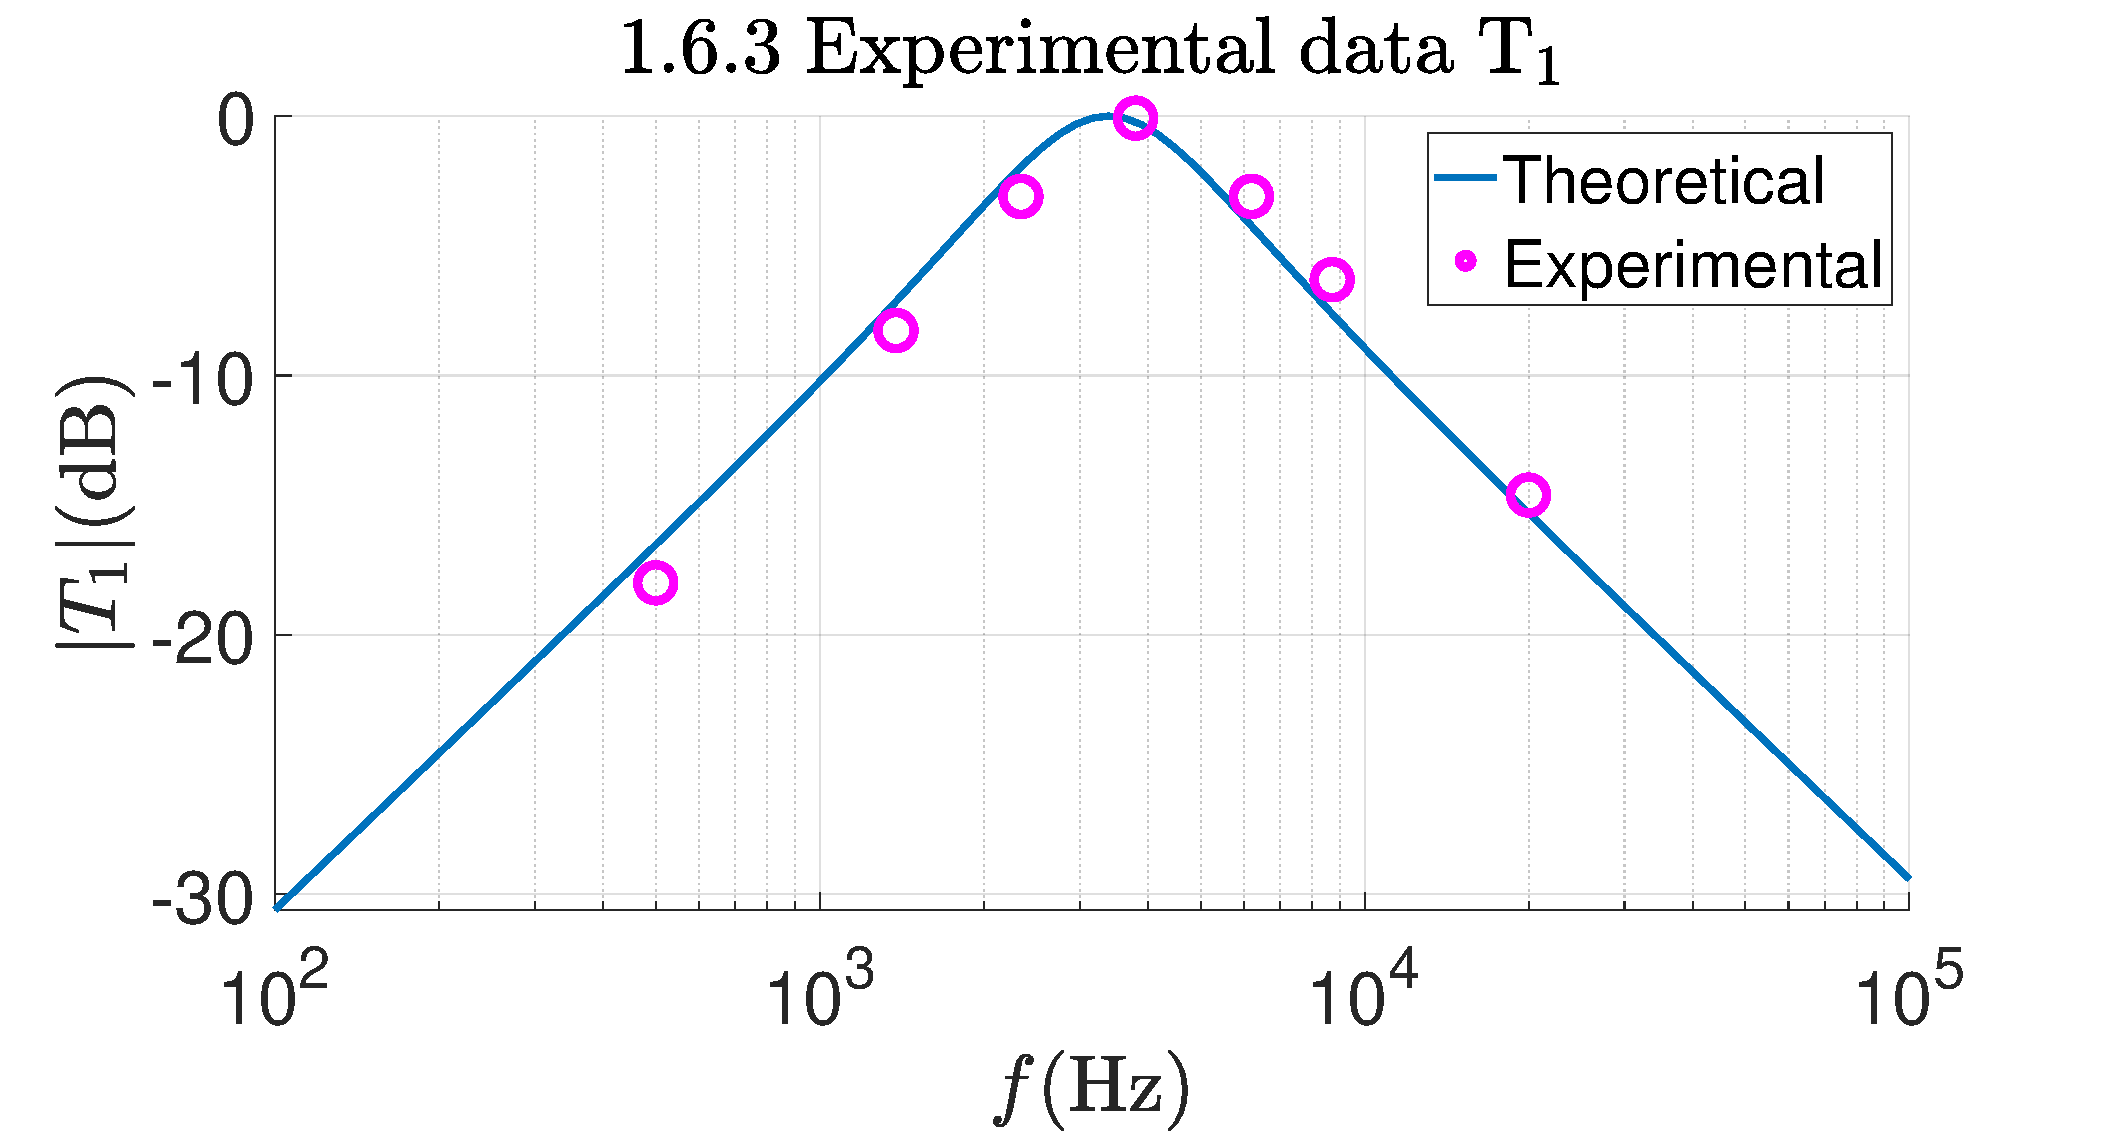
\includegraphics[width=\textwidth]{Imagens/1_6_3_bodeExperimental1.pdf}
         \caption{Filtro $T_1$.}
         \label{fig:bode_exp_TT_P2_10kohm_T1}
     \end{subfigure}
     \hfill
     \begin{subfigure}[b]{0.45\textwidth}
         \centering
         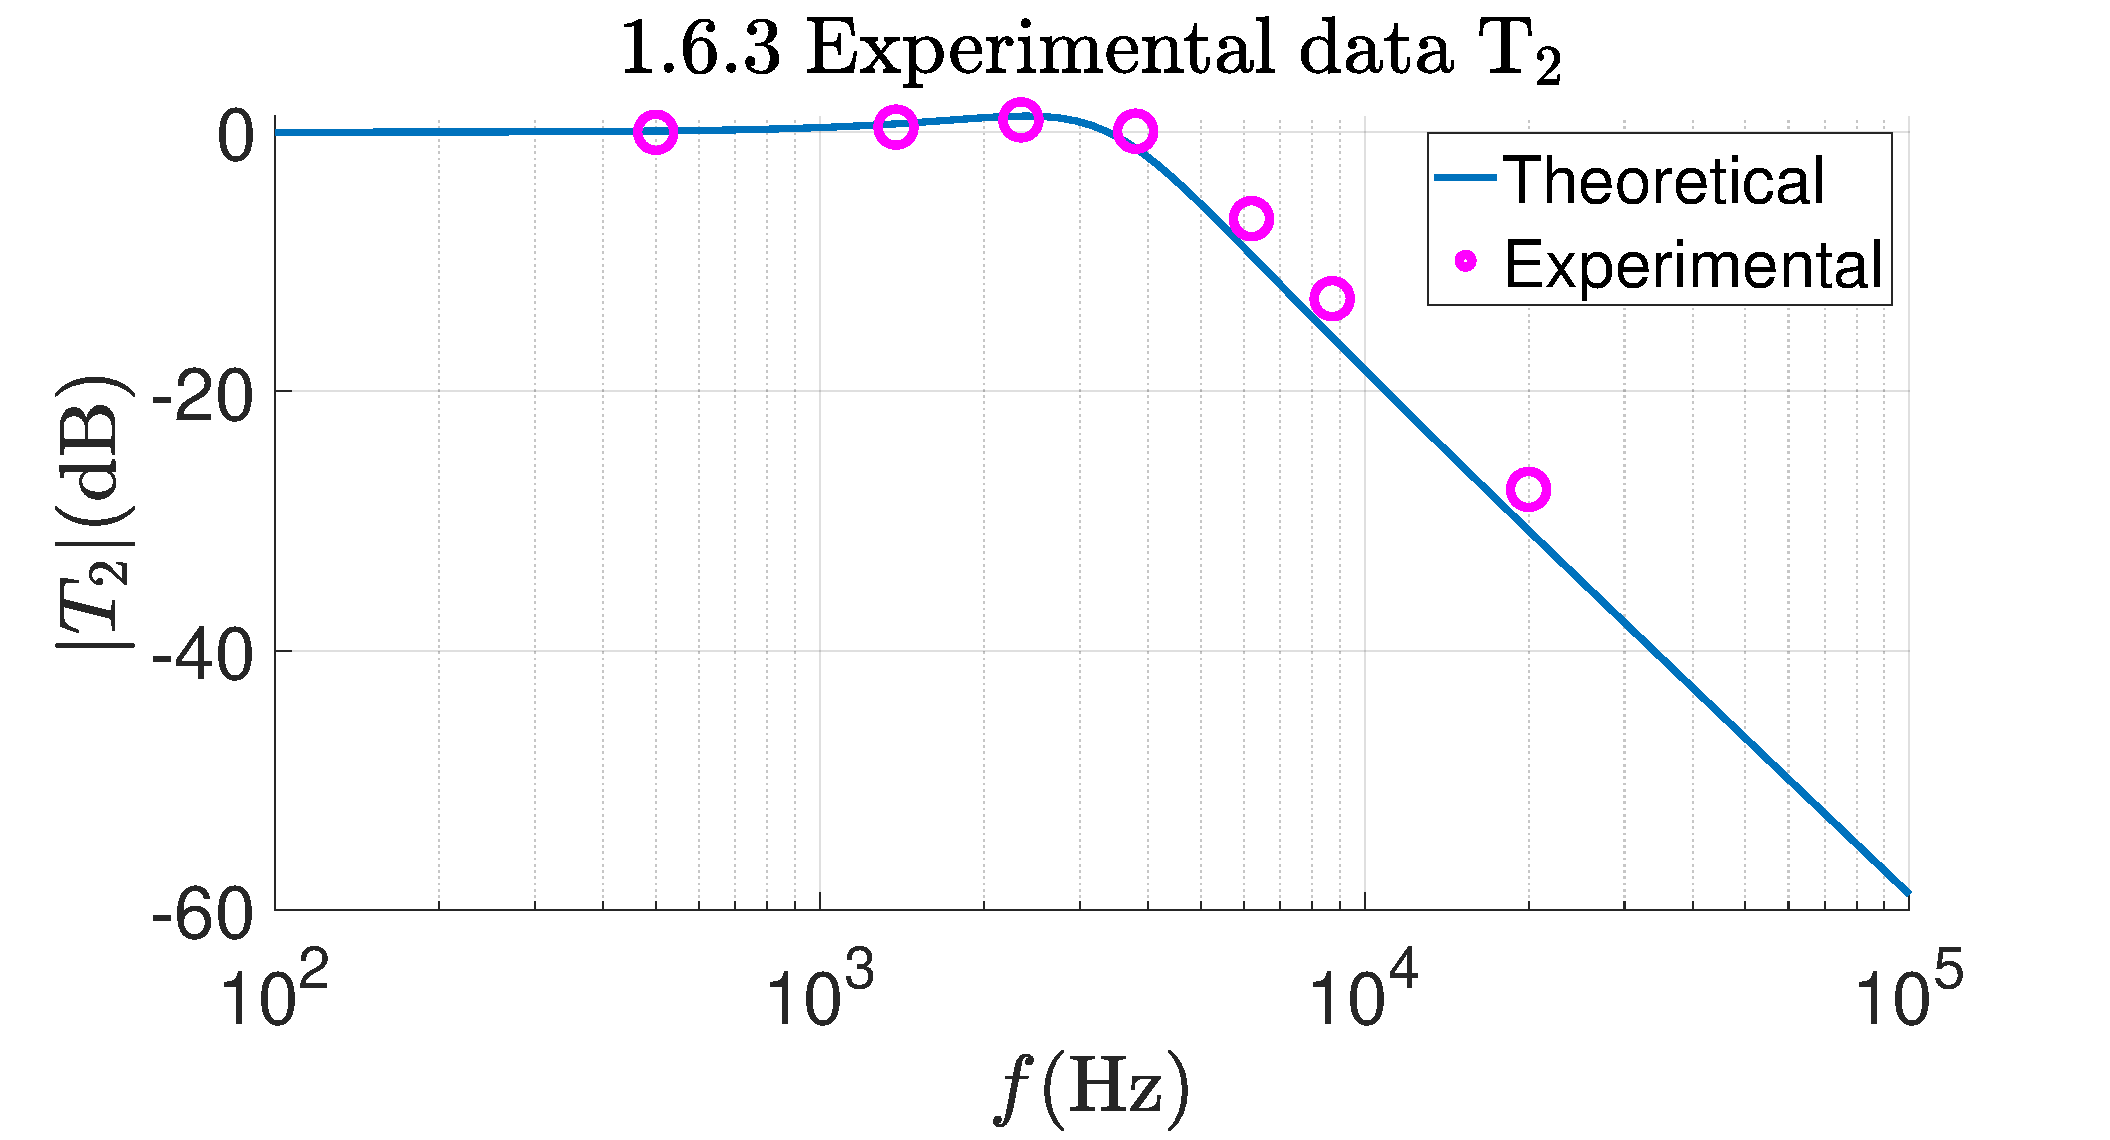
\includegraphics[width=\textwidth]{Imagens/1_6_3_bodeExperimental2.pdf}
         \caption{Filtro $T_2$.}
         \label{fig:bode_exp_TT_P2_10kohm_T2}
     \end{subfigure}
     \begin{subfigure}[b]{0.45\textwidth}
         \centering
         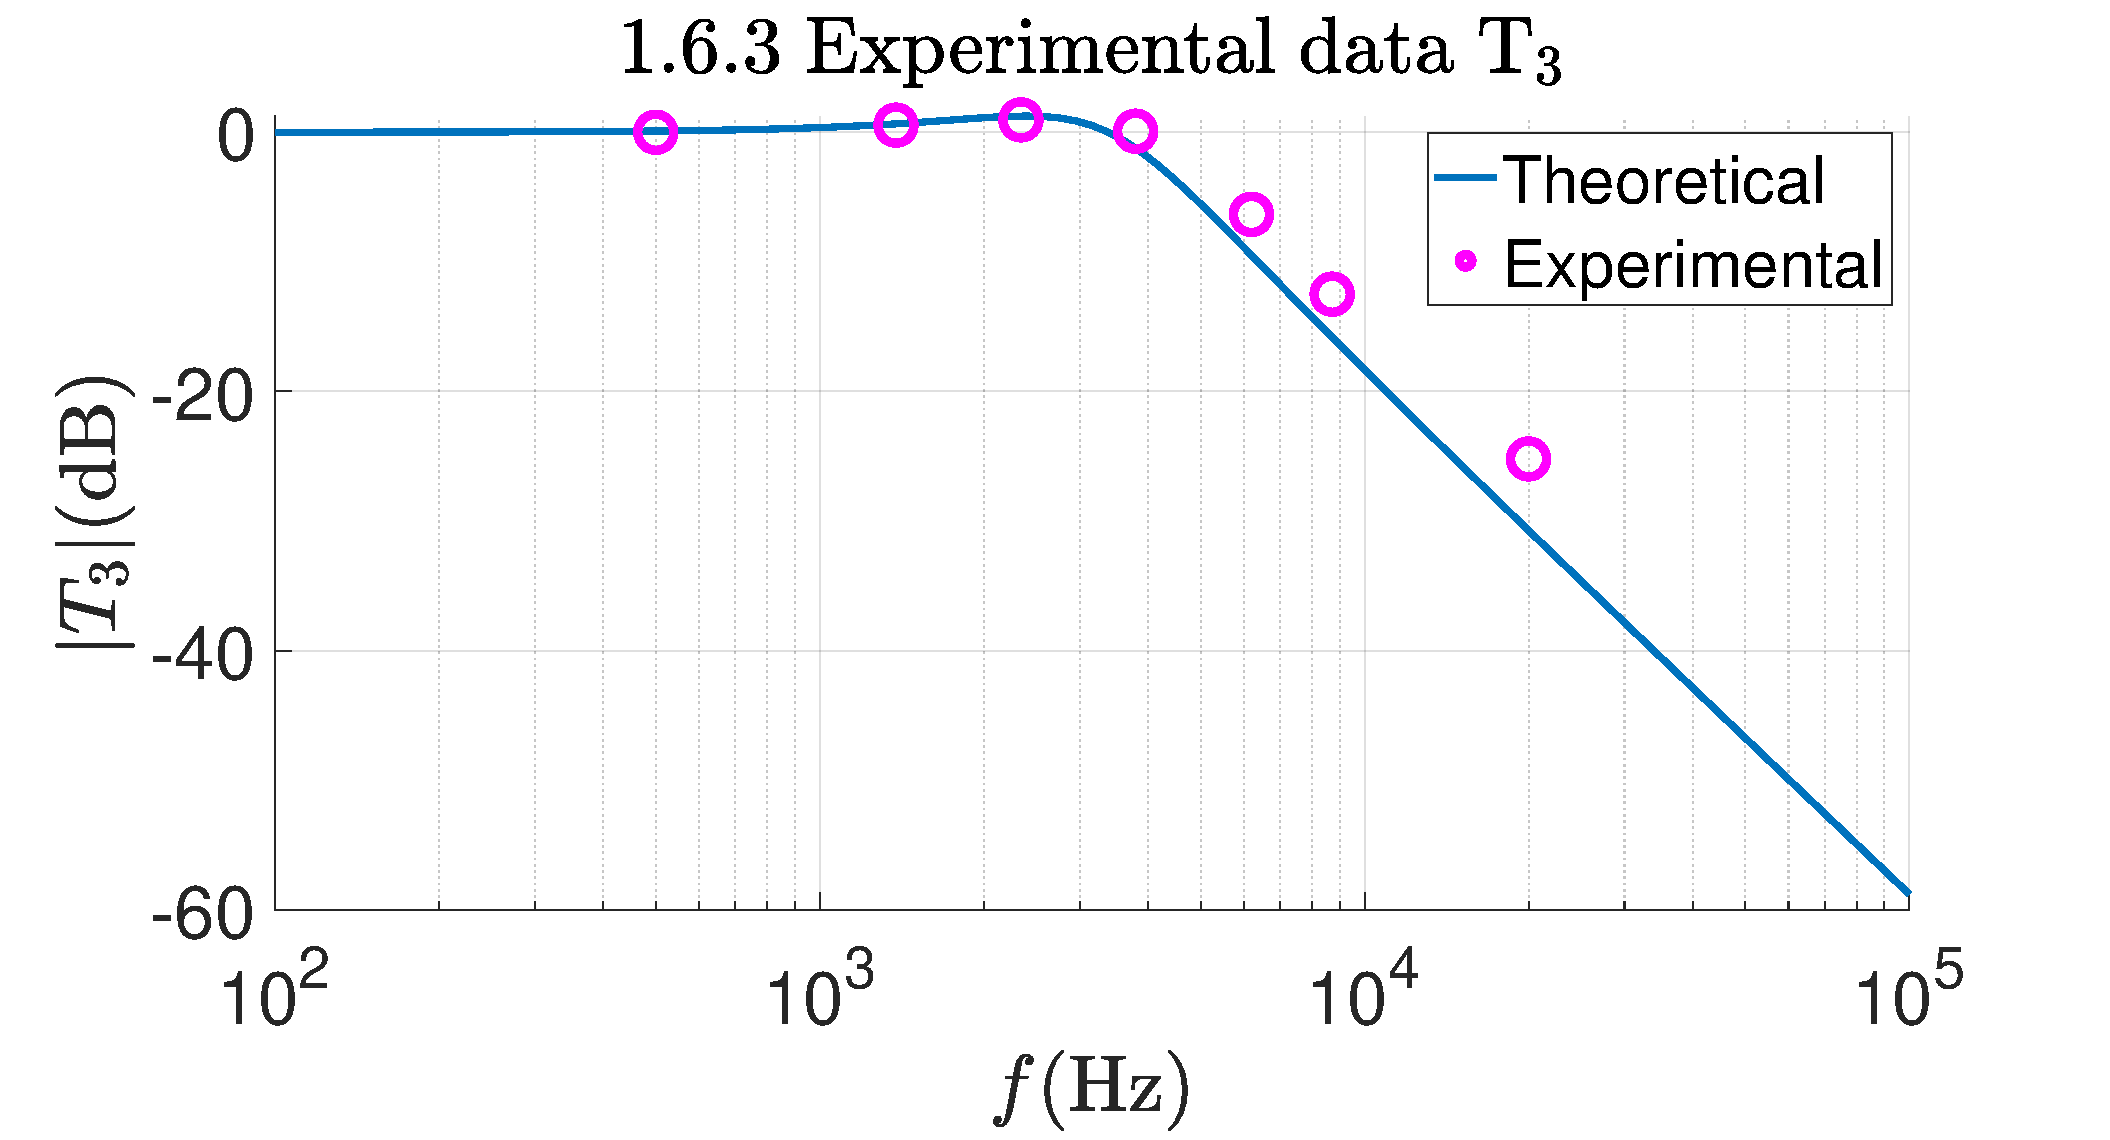
\includegraphics[width=\textwidth]{Imagens/1_6_3_bodeExperimental3.pdf}
         \caption{Filtro $T_3$.}
         \label{fig:bode_exp_TT_P2_10kohm_T3}
     \end{subfigure}
    \hfill
    \caption{Diagramas de Bode de amplitude teóricos e experimentais para $P_2 = 10 \si{\kilo \ohm}$.}
    \label{fig:bode_exp_TT_P2_10kohm}
\end{figure}

Em segundo lugar, nota-se que, como previsto teoricamente, $T_1$ é um passa-banda e $T_2$ e $T_3$ são passa-baixo. Tal conclui-se por a baixas e altas frequências $T_1$ ter uma atenuação elevada e para uma zona de médias frequências a atenuação ser reduzida e também por tanto $T_1$ e $T_3$ terem atenuações reduzidas a baixas frequências e elevadas a altas frequências.

Em terceiro lugar, observa-se que a ordem dos filtros coincide com a esperada teoricamente. Para $T_1$, que é passa-banda, a ordem 2 determina uma diminuição de -20dB/dec para altas frequências e um aumento de 20dB/dec para baixas frequências devido à presença de um zero na origem e dois pólos à frequência central do filtro. Para $T_2$ e $T_3$, que são passa-baixos, a ordem 2 determina uma diminuição de -40dB/dec para altas frequências devido à ausência de zeros e à presença de dois pólos à frequência $f_0$. Tendo os diagramas de Bode teóricos estas variações em conta e sendo os valores experimentais idênticos aos teóricos como mostrado pela Fig. \ref{fig:bode_exp_TT_P2_10kohm}, pode-se conjeturar que a ordem é a correta. No entanto, apresenta-se também uma aproximação das diminuições por década dos ganhos. Tal aproximação baseia-se numa regressão linear, que devido à sua simplicidade não se detalhará mais, envolvendo os três maiores valores de frequência e correspondentes ganhos em dB retirados da Tabela \ref{tab:dados_bode_exp_TT}. Dessa análise, retiram-se diminuições de -22.7dB/dec, -41.0dB/dec e -36.8dB/dec para $T_1$, $T_2$ e $T_3$ respetivamente, as quais entram em linha de conta com os resultados acima mencionados.

A partir da Tabela \ref{tab:valores_teoricos_experimentais_TT}, que utiliza os valores experimentais obtidos com o primeiro método, conclui-se que os desvios dos valores teóricos em relação aos experimentais foram reduzidos para $K$, $Q$ e $G$. O maior ocorreu para $\omega_0$ sendo de 12.2\% do valor teórico. Esta diferença é razoável quando se consideram a elevada tolerância de $C_2$ e a tolerância de 5\% de $R_{11}$. 

\begin{table}[h!]
    \centering
    \caption{Valores teóricos e experimentais de $K$, $G$, $Q$ e $\omega_0$.}
    \label{tab:valores_teoricos_experimentais_TT}
    \begin{tabular}{cccc}
    \hline
    Parâmetro & Valor experimental & Valor teórico & Erro relativo \\
    \hline  
    $K$ & 1.00  & 1.00  & 0.00\% \\
    $G$ & 1.00  & 1.00  & 0.00\% \\
    $Q$ & 1.00  & 0.991  & -0.900\% \\
    $\omega_0 [\si{\radian\per\second}]$ & $21.3 \times 10^3$ & $23.9 \times 10^3$ & 12.2\% \\
    \hline
    \end{tabular}
\end{table}

Tendo agora em conta a influência do valor de $P_2$, observa-se, tal como previsto teoricamente, que não existe alteração do fator de qualidade, $Q$, e que $K$ varia de acordo com \eqref{eq:KTT}. K varia de acordo com \eqref{eq:KTT}, pois, como apresentado em \ref{tab:influencia_P2_TT_V2}, o ganho do filtro $T_2$ a baixa frequência, que corresponde a $K$, é aproximadamente igual a $R_4/P_2$. Para além disso, $Q$ não se altera, porque, de acordo com \ref{tab:influencia_P2_TT_V1}, as alterações no ganho de $T_1$ à frequência central são apenas as devidas à alteração de $K$.

\subsection{Conclusões}

Nesta sessão de laboratório, estudou-se a realização de filtros RC ativos através da secção biquadrática de Tow-Thomas e da secão biquadrática de Kerwin, Huelsman e Newcomb. Pôde-se observar as caraterísticas experimentais de resposta das duas montagens de três amplificadores operacionais e como elas se desviam dos resultados teóricos, nomeadamente o tipo de filtragem, a ordem do filtro, as frequências importantes dos diagramas de Bode dos filtros e os parâmetros da resposta.

Na montagem KHN, trabalhámos com filtros de 2ª ordem: um filtro passa-alto ($T_1$), um filtro passa-banda ($T_2$), e um filtro passa-baixo ($T_3$), como previsto teoricamente. Comparando os resultados experimentais com os resultados teóricos, os parâmetros $K$, $Q$ apresentaram erros muito baixos, sendo $\omega_0$ o parâmetro com o maior erro associado. Relativamente à influência do divisor de tensão variável na montagem, concluímos e comprovámos que afeta ambos os parâmetros $K$ e $Q$ de maneira diferente. $K$ varia parabolicamente com o valor de $R_g$, sendo o valor de $K$ igual para valores complementares. Em relação a $Q$, há uma diminuição com o aumento de ${R_g}/{P_2}$.

É de notar quanto à montagem TT que os tipos de filtragem correspondem aos esperados teoricamente, sendo $T_1$ um passa-banda, $T_2$ um passa-baixo, e $T_3$ um passa-baixo. Foi também importante observar que todos os filtros se comportam experimentalmente como de 2ª ordem. Para além disso, os valores dos parâmetros da resposta experimentais também estão muito próximos dos teóricos, com exceção de $\omega_0$. Considera-se que este desvio experimental de $\omega_0$ se deve à tolerância de componentes do circuito. Quanto à variação do valor de $P_2$ verificou-se que ela apenas afetava o valor de $K$ e não de $Q$. De  facto, $K$ é inversamente proporcional a $P_2$ com constante $R_4$.

\clearpage